\documentclass[12pt,a4paper]{article}
\usepackage[utf8]{inputenc}
\usepackage[T1]{fontenc}
\usepackage[provide=*,french]{babel}
\usepackage{graphicx}
\usepackage{geometry}
\usepackage{hyperref}
\usepackage[all]{hypcap}

\geometry{margin=2.5cm}

\begin{document}

% Page de garde
\begin{titlepage}
    \begin{center}
        \vspace*{2cm}
        {\huge\bfseries Devoir 3\par}
        {INFO4305\par}
        \vspace{2cm}
        {\Large Alec Jones\par}
        {\large A00216262\par}
        \vfill
    \end{center}
\end{titlepage}

\tableofcontents
\newpage

% Introduction
\section{Introduction}

% Objectif
\section{Objectif du TP}
 [Les objectifs du TP]

% Corps du rapport
\newpage
\section{Déroulement du TP}
\subsection{Partie 1}
Premièrement on doit d'abord installer Gpg4win, j'ai installer le logiciel à
l'aide du manager de paquets WinGet (voir la figure \ref{gpg4win}).

\begin{figure}[h]
    \centering
    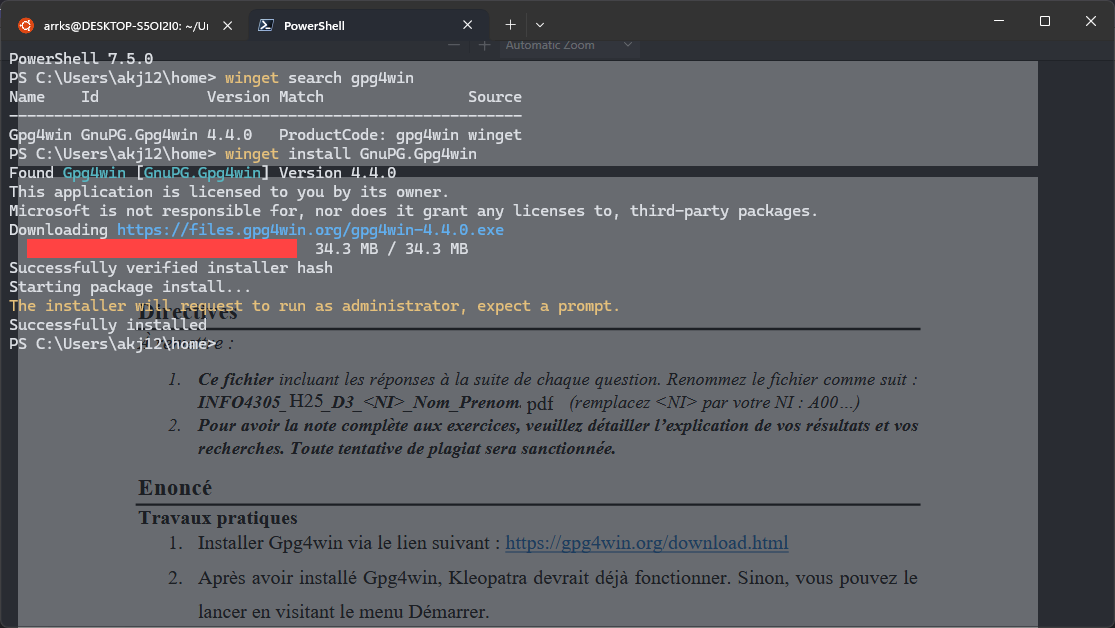
\includegraphics[width=0.8\textwidth]{../img/gpg4win.png}
    \caption{Installation de Gpg4win}
    \label{gpg4win}
\end{figure}

\subsection{Partie 2}
\subsubsection{Partie a}
Pour créer une paire de clé à l'aide de l'interface graphique, on doit ouvirir le logiciel
Kleopatra, ensuite on selectionne l'option new key pair (voir la figure \ref{kleopatra}).

\begin{figure}[h]
    \centering
    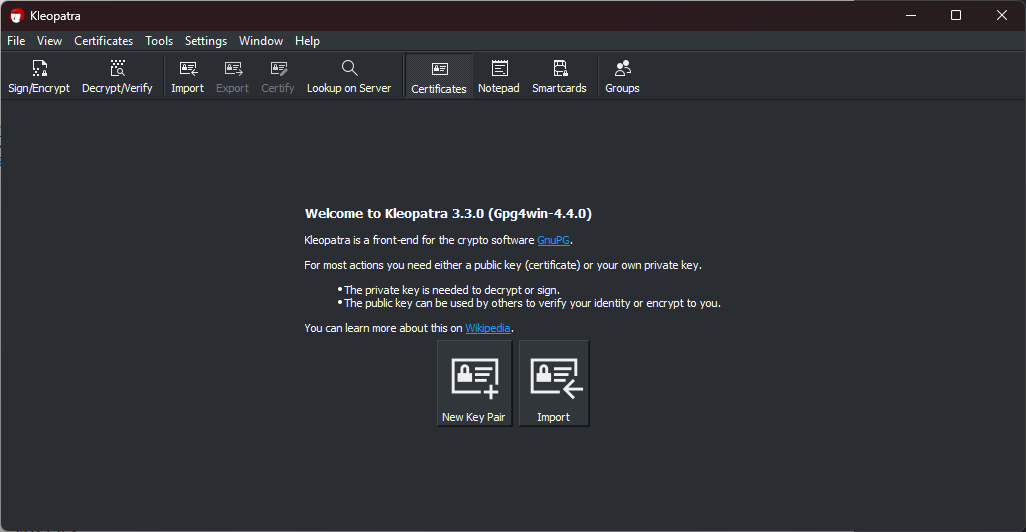
\includegraphics[width=0.8\textwidth]{../img/kleopatra.png}
    \caption{Menu initial Kleopatra}
    \label{kleopatra}
\end{figure}

Ensuite, on doit sélectionné options avancés et puis rsa2048.
On doit aussi remplir notre nom et notre courriel pour le certificat (voir \ref{newKey}).

\begin{figure}[ht]
    \centering
    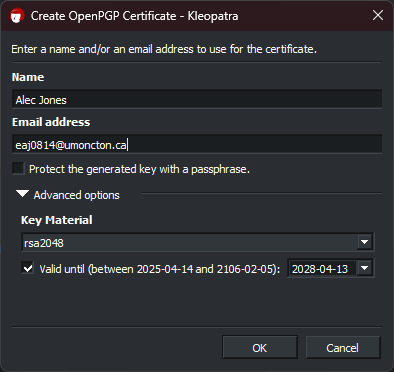
\includegraphics[width=0.8\textwidth]{../img/newKey.png}
    \caption{Création de clés dans Kleopatra}
    \label{newKey}
\end{figure}

\subsubsection{Partie b}


% Conclusion
\section{Observation, interprétation et conclusion}
 [Vos observations et conclusions]
\begin{itemize}
    \item Objectifs atteints ou non
    \item Ce que vous avez accompli
    \item Ce que vous avez compris
\end{itemize}

\end{document}
